% =====================================================================
\section{Conservative Vector Fields and Potential Functions}\label{ch:conservative}
% =====================================================================

\subsection{Definition}

Some vector fields can be represented as the gradients of differentiable
functions and some cannot. Those that can are called \emph{conservative}
(Slides).

\begin{definition}[Conservative field; Slides, Definition 4]\label{def:conservative}
A vector field $\vF$ is called \emph{conservative} when there exists a
differentiable function $f$ such that $\vF=\grad f$. The function $f$ is called a
\emph{potential function} for $\vF$.
\end{definition}

\begin{remark}
(1) If $f$ is a potential for $\vF$, so is $f+C$ for every constant $C$, since
$\grad C=\vzero$. On a connected domain these are \emph{all} the potentials, so
the answer to ``find the potential'' is always ``$f+C$''.
(2) The name comes from physics: for a conservative force, mechanical energy
is conserved. Physicists usually write $\vF=-\grad U$, with $U=-f$ the
\emph{potential energy}; e.g.\ gravity is $\grad(mMG/r)$ (Example~\ref{ex:gradfield3}).
\end{remark}

\begin{example}[Slides, Example 7.3]\label{ex:7.3}
The vector field $\vF(x,y)=\ip{3x^2,\,y}$ is conservative, since
$f(x,y)=x^3+\frac12y^2$ satisfies $\grad f=\ip{3x^2,\,y}=\vF$.
\end{example}
\begin{solution}
Verification: $f_x=3x^2$ and $f_y=\frac12\cdot2y=y$, so $\grad f=\vF$.\checkok
How was $f$ found? Each component depends on one variable only, so
$f=\int3x^2\,\dd x+\int y\,\dd y=x^3+\frac12y^2$ (plus a constant). The general
method is in Section~\ref{sec:potential}.
\end{solution}

\subsection{Why there is a test: mixed partials}

Suppose $\vF=\ip{M,N}=\grad f$, i.e.\ $M=f_x$ and $N=f_y$, where $f$ has
continuous second partial derivatives. Then by Clairaut's theorem
(Theorem~\ref{thm:clairaut})
\[
  M_y=(f_x)_y=f_{xy}=f_{yx}=(f_y)_x=N_x .
\]
So $M_y=N_x$ is a \emph{necessary} condition for $\ip{M,N}$ to be conservative.
On a disk (or any simply connected region) it is also \emph{sufficient}.

\begin{theorem}[Test for conservative vector field in the plane; Slides, Theorem 1]\label{thm:test2}
Let $M$ and $N$ have continuous first partial derivatives on an open disk $R$.
The vector field $\vF(x,y)=M\,\vi+N\,\vj$ is conservative on $R$ if and only if
\[
  \pd{N}{x}=\pd{M}{y}\qquad(\text{i.e. } N_x=M_y).
\]
\end{theorem}

\begin{example}[Slides, Example 7.4]\label{ex:7.4}
Determine whether the vector field is conservative:
(1) $\vF(x,y)=\ip{x^3y,\,xy}$;\quad (2) $\vF(x,y)=\ip{2x,\,y}$.
\end{example}
\begin{solution}
\textbf{(1)} $M=x^3y$, $N=xy$: $M_y=x^3$ and $N_x=y$. These are not equal (e.g.\ at
$(1,0)$: $1\neq0$), so $\vF$ is \textbf{not} conservative.

\textbf{(2)} $M=2x$, $N=y$: $M_y=0=N_x$. The partials are continuous on all of
$\R^2$, so $\vF$ \textbf{is} conservative. (Indeed $f=x^2+\frac12y^2$.)
\end{solution}

\begin{warning}
$M_y=N_x$ must hold as an \emph{identity}, for all $(x,y)$ in the region, not
just at one point. In (1), $x^3=y$ holds along a curve, but that does not
make $\vF$ conservative.
\end{warning}

\begin{theorem}[Test for conservative vector field in space; Slides, Theorem 2]\label{thm:test3}
Let $M$, $N$ and $P$ have continuous first partial derivatives on an open
sphere (ball) $Q$. The vector field $\vF(x,y,z)=M\,\vi+N\,\vj+P\,\vk$ is
conservative on $Q$ if and only if
\[
  M_y=N_x,\qquad N_z=P_y,\qquad P_x=M_z .
\]
\end{theorem}

\begin{remark}[Remembering the three conditions]
Each condition pairs two components and two variables: the
$(x,y)$-pair $M_y=N_x$, the $(y,z)$-pair $N_z=P_y$, the $(z,x)$-pair $P_x=M_z$.
They come from $f_{xy}=f_{yx}$, $f_{yz}=f_{zy}$, $f_{zx}=f_{xz}$. (They say that
the \emph{curl} of $\vF$, $\ip{P_y-N_z,\,M_z-P_x,\,N_x-M_y}$, is zero.)
\end{remark}

\begin{example}[Slides, Example 7.5]\label{ex:7.5}
Determine whether the vector field is conservative:
\[
  \vF(x,y,z)=\frac{x}{x^2+y^2+z^2}\,\vi+\frac{y}{x^2+y^2+z^2}\,\vj+\frac{z}{x^2+y^2+z^2}\,\vk .
\]
\end{example}
\begin{solution}
Write $\rho=x^2+y^2+z^2$, so $M=x/\rho$, $N=y/\rho$, $P=z/\rho$. Quotient rule,
remembering that the numerator of $M$ does not involve $y$ or $z$, etc.:

\step{1}{$M_y$ and $N_x$.}
\[
  M_y=\frac{\rho\cdot0-x\cdot2y}{\rho^2}=\frac{-2xy}{\rho^2},\qquad
  N_x=\frac{\rho\cdot0-y\cdot2x}{\rho^2}=\frac{-2xy}{\rho^2}.\qquad\text{So }M_y=N_x.
\]
\step{2}{$N_z$ and $P_y$.}
\[
  N_z=\frac{\rho\cdot0-y\cdot2z}{\rho^2}=\frac{-2yz}{\rho^2},\qquad
  P_y=\frac{\rho\cdot0-z\cdot2y}{\rho^2}=\frac{-2yz}{\rho^2}.\qquad\text{So }N_z=P_y.
\]
\step{3}{$P_x$ and $M_z$.}
\[
  P_x=\frac{-2xz}{\rho^2},\qquad M_z=\frac{-2xz}{\rho^2}.\qquad\text{So }P_x=M_z.
\]
By Theorem~\ref{thm:test3}, $\vF$ is conservative, i.e. a potential function
$f$ with $\grad f=\vF$ exists. (By Example~\ref{ex:gradfield3}(a),
$f=\frac12\ln(x^2+y^2+z^2)+C$; the slides derive it in Example~7.6 below.)
\end{solution}

\begin{remark}[About the domain]
$\vF$ is undefined at the origin, so strictly its domain is
$\R^3\setminus\{\vzero\}$, not an open ball. The conclusion is still correct:
the test works on any \emph{simply connected} region, and $\R^3$ minus a point is
simply connected (every loop can be shrunk to a point while avoiding the
origin). On every ball not containing the origin, Theorem~\ref{thm:test3}
applies directly.
\end{remark}

\subsection{Finding a potential function}\label{sec:potential}

If $\vF=\ip{M,N,P}$ is conservative, there is $f$ with
$\ip{f_x,f_y,f_z}=\ip{M,N,P}$, i.e.
\[
  f_x=M,\qquad f_y=N,\qquad f_z=P .
\]
We find $f$ by \emph{reversing partial differentiation}: integrate one equation
and use the other two to determine the missing function (Slides).

\begin{strategy}{Strategy (finding the potential function; Slides).}
\begin{enumerate}
\item \textbf{Integrate with respect to $x$.} From $f_x=M$:
      \[ f(x,y,z)=\int M\,\dd x+g(y,z), \]
      where $g(y,z)$ is (at this point) an unknown function.
\item \textbf{Differentiate with respect to $y$.} Differentiate the $f$ from
      Step~1 with respect to $y$ and set $f_y=N$. Solve for $g_y(y,z)$, then
      integrate with respect to $y$. This determines $g(y,z)$ up to an unknown
      function $h(z)$.
\item \textbf{Differentiate with respect to $z$.} Substitute $g$ into $f$,
      differentiate with respect to $z$ and set $f_z=P$. Solve for $h'(z)$,
      then integrate to obtain $h(z)$.
\item \textbf{Assemble and check} $\grad f=\vF$. Answer: $f+C$.
\end{enumerate}
In two variables stop after Step~2, with $g=g(y)$ a function of $y$ only, whose
derivative $g'(y)$ is found from $f_y=N$.
\end{strategy}

\begin{remark}[A built-in alarm]
In Step~2, $g_y$ must turn out to depend on $y$ and $z$ only (and in Step~3,
$h'$ on $z$ only). If an $x$ survives, either you made an algebra error or $\vF$
is not conservative (Example~\ref{ex:not-cons}).
\end{remark}

\begin{example}[Two variables]\label{ex:pot2d}
Show that $\vF(x,y)=\ip{3+2xy,\;x^2-3y^2}$ is conservative and find a potential
function.
\end{example}
\begin{solution}
\step{1}{Test.} $M_y=2x$ and $N_x=2x$; the partials are continuous on $\R^2$,
so $\vF$ is conservative.
\step{2}{Integrate $f_x=M$ in $x$.} $f=\int(3+2xy)\,\dd x=3x+x^2y+g(y)$.
\step{3}{Use $f_y=N$.} $f_y=x^2+g'(y)$ must equal $x^2-3y^2$, so $g'(y)=-3y^2$ (no
$x$: good) and $g(y)=-y^3+K$.
\step{4}{Answer.} $f(x,y)=3x+x^2y-y^3+K$.
\step{5}{Check.} $f_x=3+2xy$\checkok, $f_y=x^2-3y^2$\checkok.
\end{solution}

\begin{example}[Slides, Example 7.6]\label{ex:7.6}
Find the potential function for
$\vF(x,y,z)=\dfrac{x}{x^2+y^2+z^2}\,\vi+\dfrac{y}{x^2+y^2+z^2}\,\vj+\dfrac{z}{x^2+y^2+z^2}\,\vk$.
\end{example}
\begin{solution}
$\vF$ is conservative by Example~\ref{ex:7.5}.

\step{1}{Integrate with respect to $x$.} $f_x=M=\dfrac{x}{x^2+y^2+z^2}$. Substituting
$w=x^2+y^2+z^2$, $\dd w=2x\,\dd x$ ($y,z$ fixed):
\[
  f(x,y,z)=\int\frac{x}{x^2+y^2+z^2}\,\dd x=\frac12\ln\abs{x^2+y^2+z^2}+g(y,z).
\]
\step{2}{Differentiate with respect to $y$.}
\[
  f_y=\frac12\cdot\frac{2y}{x^2+y^2+z^2}+g_y(y,z)=\frac{y}{x^2+y^2+z^2}+g_y(y,z).
\]
Comparing with $f_y=N=\dfrac{y}{x^2+y^2+z^2}$ gives $g_y(y,z)=0$. Integrating with
respect to $y$: $g(y,z)=\int0\,\dd y=C_1+h(z)$ for some constant $C_1$ and some
function $h(z)$. Hence
\[
  f(x,y,z)=\frac12\ln\abs{x^2+y^2+z^2}+C_1+h(z).
\]
\step{3}{Differentiate with respect to $z$.}
$f_z=\dfrac{z}{x^2+y^2+z^2}+h'(z)$. Comparing with $f_z=P=\dfrac{z}{x^2+y^2+z^2}$ gives
$h'(z)=0$, so $h(z)=\int0\,\dd z=C_2$. Hence
\[
  f(x,y,z)=\tfrac12\ln\abs{x^2+y^2+z^2}+C_1+C_2 .
\]
\textbf{Answer.} The potential function is of the form
\[
  f(x,y,z)=\frac12\ln\left(x^2+y^2+z^2\right)+C,
\]
$C$ an arbitrary constant. (The absolute value can be dropped since
$x^2+y^2+z^2>0$ on the domain.)
\end{solution}

\begin{exercise}[Slides, Exercise 4]\label{ex:exercise4}
Determine whether $\vF(x,y,z)=y^2\,\vi+(2xy+e^{3z})\,\vj+3ye^{3z}\,\vk$ is
conservative. If it is, find a potential function for $\vF$.
\end{exercise}
\begin{solution}
$M=y^2$, $N=2xy+e^{3z}$, $P=3ye^{3z}$.

\step{1}{Test (Theorem~\ref{thm:test3}).}
\[
  M_y=2y=N_x,\qquad N_z=3e^{3z}=P_y,\qquad P_x=0=M_z .
\]
All partials are continuous on $\R^3$, so $\vF$ \textbf{is conservative}.

\step{2}{Integrate $f_x=y^2$ in $x$.} $f=xy^2+g(y,z)$.

\step{3}{Differentiate in $y$.} $f_y=2xy+g_y(y,z)$. Setting equal to
$N=2xy+e^{3z}$: $g_y(y,z)=e^{3z}$. Integrate in $y$ ($z$ fixed):
$g(y,z)=ye^{3z}+h(z)$. So $f=xy^2+ye^{3z}+h(z)$.

\step{4}{Differentiate in $z$.} $f_z=3ye^{3z}+h'(z)$. Setting equal to
$P=3ye^{3z}$: $h'(z)=0$, $h(z)=C$.

\textbf{Answer.} $f(x,y,z)=xy^2+ye^{3z}+C$.

\step{5}{Check.} $\grad f=\ip{y^2,\;2xy+e^{3z},\;3ye^{3z}}=\vF$.\checkok
\end{solution}

\begin{example}\label{ex:pot3d}
Find a potential for $\vF=\ip{2xy+z^2,\;x^2,\;2xz+\cos z}$.
\end{example}
\begin{solution}
\step{1}{Test.} $M_y=2x=N_x$; $N_z=0=P_y$; $P_x=2z=M_z$. Conservative on $\R^3$.
\step{2}{$x$-integration.} $f=x^2y+xz^2+g(y,z)$.
\step{3}{$y$.} $f_y=x^2+g_y=x^2\Rightarrow g_y=0\Rightarrow g=h(z)$.
\step{4}{$z$.} $f_z=2xz+h'(z)=2xz+\cos z\Rightarrow h'(z)=\cos z\Rightarrow h=\sin z+C$.

\textbf{Answer.} $f=x^2y+xz^2+\sin z+C$. Check: $\grad f=\ip{2xy+z^2,\,x^2,\,2xz+\cos z}$.\checkok
\end{solution}

\begin{example}[What goes wrong if $\vF$ is not conservative]\label{ex:not-cons}
Try to find a potential for $\vF=\ip{x^3y,\;xy}$ (Example~\ref{ex:7.4}(1)).
\end{example}
\begin{solution}
Step~1 gives $f=\frac14x^4y+g(y)$. Step~2: $f_y=\frac14x^4+g'(y)$ should equal $xy$, so
$g'(y)=xy-\frac14x^4$. But $g'(y)$ is supposed to depend on $y$ only, and the
right-hand side depends on $x$. Contradiction: no potential exists, in
agreement with the test $M_y=x^3\neq y=N_x$.
\end{solution}

\begin{remark}[A quick alternative for checking]
Integrate each component in its own variable and merge the terms:
$\int M\,\dd x$, $\int N\,\dd y$, $\int P\,\dd z$, keeping every distinct term
once. For Exercise~4: $\int y^2\,\dd x=xy^2$, $\int(2xy+e^{3z})\,\dd y=xy^2+ye^{3z}$,
$\int3ye^{3z}\,\dd z=ye^{3z}$; merging gives $xy^2+ye^{3z}$. This is fast but
\emph{must} be followed by the check $\grad f=\vF$, because it can silently
produce a wrong answer when $\vF$ is not conservative. On an exam, show the
three-step method.
\end{remark}

\subsection{A caveat: the shape of the domain}\label{sec:caveat}

Theorems~\ref{thm:test2} and~\ref{thm:test3} are stated on a disk or a ball.
They remain true on any simply connected region, but can fail on regions with
holes.

\begin{example}[The vortex field]\label{ex:vortex}
Let $\vF(x,y)=\dfrac{-y}{x^2+y^2}\,\vi+\dfrac{x}{x^2+y^2}\,\vj$ on the punctured
plane $\R^2\setminus\{(0,0)\}$. Show that $M_y=N_x$ everywhere on this domain.
\end{example}
\begin{solution}
\[
  M_y=\frac{(x^2+y^2)(-1)-(-y)(2y)}{(x^2+y^2)^2}=\frac{y^2-x^2}{(x^2+y^2)^2},\qquad
  N_x=\frac{(x^2+y^2)(1)-x(2x)}{(x^2+y^2)^2}=\frac{y^2-x^2}{(x^2+y^2)^2}.
\]
They agree. Nevertheless, $\vF$ is \emph{not} conservative on the punctured
plane. Suppose, for contradiction, that $\vF=\grad f$ there. Walk once around
the unit circle, $\vr(t)=\ip{\cos t,\sin t}$, and let $g(t)=f(\cos t,\sin t)$.
By the chain rule (Lecture Notes No.~6, Theorem~1.11),
\[
  g'(t)=\grad f(\vr(t))\cdot\vr\,'(t)=\vF(\cos t,\sin t)\cdot\ip{-\sin t,\cos t}
  =\ip{-\sin t,\cos t}\cdot\ip{-\sin t,\cos t}=1 ,
\]
using $x^2+y^2=1$ on the circle. Hence $g(2\pi)-g(0)=\int_0^{2\pi}1\,\dd t=2\pi$.
But $\vr(2\pi)=\vr(0)$ is the same point, so $g(2\pi)=g(0)$: a contradiction.
The hole at the origin is responsible (Figure~\ref{fig:vortex}).

On the right half-plane $x>0$ (simply connected), $\vF=\grad\theta$ with
$\theta=\arctan(y/x)$ the polar angle (Lecture Notes No.~6,
Problem~5.11). Going once around the origin, the angle increases by $2\pi$ and
cannot return to its starting value; that is why no single potential exists
on the whole punctured plane.
\end{solution}

\begin{figure}[H]
  \centering
  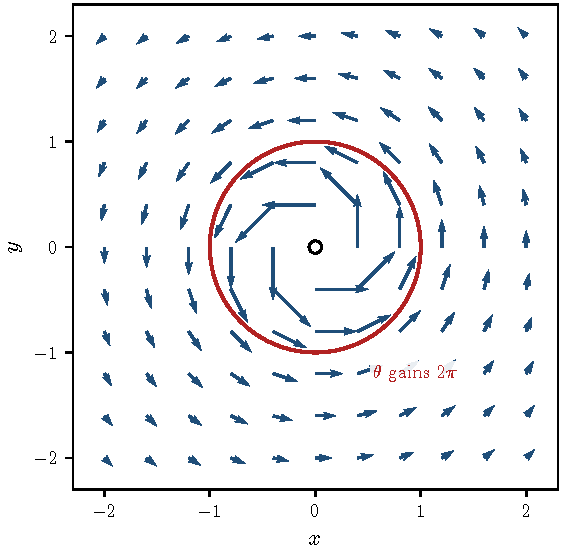
\includegraphics[width=0.46\linewidth]{vortex}
  \caption{The vortex field (arrow lengths capped near the origin). $M_y=N_x$
  everywhere, yet a would-be potential would have to increase by $2\pi$ on each
trip around the red circle, which is impossible.}
  \label{fig:vortex}
\end{figure}

\begin{keybox}{Summary: deciding and finding}
\begin{enumerate}
\item Compute the cross partials ($M_y,N_x$ in 2D; all three pairs in 3D).
\item If any pair differs: \textbf{not conservative}. Stop.
\item If all pairs agree and the domain is a disk/ball/all of $\R^n$ (or simply
      connected): \textbf{conservative}. Find $f$ by the three-step method and
      check $\grad f=\vF$.
\end{enumerate}
\end{keybox}
